Our second contribution is to minimize the above heterogeneity using the
Charm++ load balancers.  We first observed the working of existing load
balancers like \emph{RefineLB} \& \emph{GreedyLB} to evaluate the its effect in
minimizing the heterogeneity. 
 
\subsection{Existing Load-balancers} Load balancing is a technique of
distributing computational and communication load evenly across processors of a
parallel machine so that no single processor is overloaded.  Charm++ implements
a generic, measurement-based load balancing framework which automatically
instruments all Charm++ objects, collects computation load and communication
structure during execution and stores them into a load balancing database.
Charm++ then provides a collection of load balancing strategies whose job it is
to decide on a new mapping of objects to processors based on the information
from the database.  These strategies work under the assumption that objects in
a Charm++ application tend to exhibit temporal correlation in their computation
and communication patterns, i.e. future can be predicted to some extent using
the collected data, allowing effective measurement-based load balancing without
application-specific knowledge. Following are the two widely used load
balancing strategies:

\subsubsection{RefineLB}
The objective of this strategy is to move objects away from the most overloaded
processors to reach an average. Following is the pseudo-algorithm of this
strategy:

\begin{algorithm}
 \KwData{V$_t$:(the set of objects; V$_p$ (the set of processors)}
 \KwResult{Map:V$_t \rightarrow $ V$_p$ (An object mapping) }
 // build heap \;
  ProcessorHeap heavyProcs(V$_p$)\;
  Set *lightProcs\;
  \While{!done} {
    donor =   heavyProcessors$\rightarrow$deleteMax()\;
    \While{ligthProcs} {
      (obj, lightProc)  $\leftarrow$ BestObjFromDonor(donor)\;
      \If{obj.load + lightProc.load $>$ avg\_load} {
        continue\;
      } 
      \If{obj\_obtained} {
        break\;
      }
      deAssign(obj, donor)\;
      assign(obj, lightProc)\;
    }
  }
 \caption{RefineLB Pseudocode}
\end{algorithm}

 As evident from the above algorithm that it tries to migrate objects based on
 a global average which is computed as the average of each processors's load. As
 a result it restricts the number of migration which is otherwise possible.
 This restriction on object migration will be more pronounced at lower power
 caps as the opportunity for object migration is high at lower power caps due 
 to the increased heterogeneity.

\subsubsection{GreedyLB}
This uses a greedy algorithm that always assigns the heaviest object to the
least loaded processor. 

\begin{algorithm}
 \KwData{V$_t$:(the set of chare objects; \\ V$_p$ (the set of processors; \\ G$_p$ (the background load of processors) // due to non-migratable objects, etc.)}
 \KwResult{Map:V$_t \rightarrow $ V$_p$ (An object mapping) }

 // build heap of size equal to the number of objects \;
 ObjectHeap objHeap($|$V$_t|$)\;
 // insert each element of Vt in objHeap\;
 V$_t\rightarrow$objHeap \; 
 MinHeap cpuHeap(P)\;
 //Initially processors are empty with only background load\; 

 cpuHeap$\leftarrow$G$_p$\;  
 \For{ i$\leftarrow$1 to nmigobj} {
    o$\leftarrow$ objHeap.deleteMax()\;
    donor$\leftarrow$cpuHeap.deleteMin()\;
    Assign c to donor and record it in Map\;
    donor.load += c.load // add object load of c to the donor\;
    cpuHeap.insert(donor) \;
    }
 \caption{GreedyLB Pseudocode}
\end{algorithm}

The assumption for object migration is that
the time taken by the object to execute on a processor will
remain the same both before and after the migration.
This assumption is valid at higher power caps because (1) all the objects are of same
size and (2) at higher power capping values the processors are running at nearly the same 
frequencies and hence the time taken by a chare to run any of them is nearly equal.
But this assumptions fall apart at lower power caps 
because of the heterogeneity introduced between the processors and
 as a result it may happen that the object time will differ after the migration. Following is the pseudo-algorithm:

\subsection{Design: Power Aware Load Balancer}
We have established the fact that current load-balancers in charm++ are not
power aware. Current Load Balancers do not load balance based on the
individual capacity of the processor. We have also established that there is a
definite scope for improvement in execution time of the application by
minimizing the maximum idle and the average idle times of the processor.
Our motive behind the design was to make all the processors finish the
execution at the same point of time. This approach takes relative speeds of the
processors into consideration for balancing the load. We use the object times
of the chares to measure the relative speeds of the processors. We explain in
the next section, the reason to choose object time for the load balancing.  In
this approach we try to average out the execution time by assigning the load in
such a way that each of them is assigned exactly that much amount of load which
helps all the PEs finish at the same time. As it can be seen in the
Figure \ref{fig:ideal} different PEs finish execution at different points of time. As per the
motive of the design we make all the processors to finish at the same time. The
following two equations explains our design.  

\begin{figure}
\centering
\scalebox{.40} {
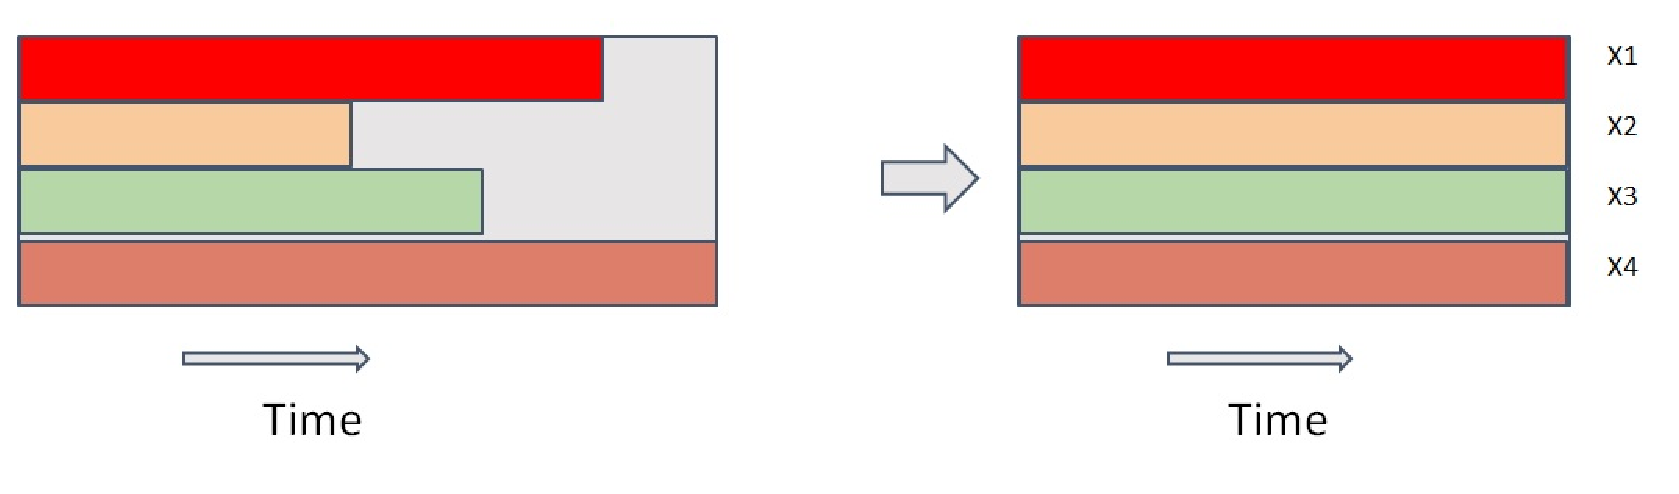
\includegraphics[scale=0.8]{Jacobi/EPS/time_diff.eps}
}
\caption{Expected Result of Power Aware Load Balancer}
\label{fig:ideal}
\end{figure}

    \begin{equation} \label{eq:3}
      (w_1x_1) = (w_2x_2) = (w_3x_3) = \dots = (w_nx_n) 
    \end{equation}
    \begin{equation} \label{eq:4}
      x_1 + x_2 + x_3 + \dots + x_n = N
    \end{equation}

  where, w$_1$, w$_2$,\dots , w$_n$ are the weights in terms of times for executing
  x$_1$, x$_2$,\dots , x$_n$ assigned objects by PE$_1$, PE$_2$,. . ., PE$_n$ 
  and $N$ is the total number of objects. 
  Before the load balancing, x$_1$, x$_2$, \dots,  x$_n$ are all the same. All the objects have
  the same load/weight in terms of computation.  Each PE executes the same
  number of objects before load balancing. Each PE before load balancing has
  the same total load since each object has the same weight. By using the above
  equation we get the proportionality based on which the number of objects will
  be assigned for the iterations after load balancing. For instance, PE1 could
  be 2 times faster than PE$_2$ and P$_3$ could be 0.5 times faster than PE$_2$. In
  which case we will have the following proportionality: PE$_1$ : PE$_1$ : PE$_3$ = 2 :
  1 : 0.5. Now based on this proportionality each PE is assigned such a load
  that everyone can finish their execution at the same point of time.  
  
  We use the second equation (\ref{eq:4}) to determine x$_1$, x$_1$, \dots,
  x$_n$. We determine x$_1$, x$_1$,
  \dots, x$_n$ values by solving for each x$_1$ up to x$_n$n by using both the
  equations. Now the determined x$_1$, x$_2$ . . . x$_n$ values is the new load
  for its respective PEs that help finish all of them at the same time. The
  newly assigned load for each of the PEs is based on the relative speeds of
  the processors. Solving the above two equations and assigning the new loads
  to the processors will now help all the processors finish at the same time.

\subsection{Selection of metric ``w''} 
We need to have a suitable metric for out parameter ``w''.  The selected metric
should demonstrate heterogeneity at the lower power caps. We have considered
processor idletime, processor overhead and processor object
time\footnote{Object time is the time taken by a charm++ object to run on a
  processor. This is also know as object walltime. Processor's object time is
    the sum of walltimes of all the objects executing on that processor} as
    candidates for our selection.  We measure these values for each processor
    id at a power cap of 24W.  Figures \ref{fig:idletime_bgtimevsproc} and
    \ref{fig:objtimevsproc} show the experimental plots.  The metric which has
    the maximum variance depicts the heterogeneity in the best possible way.
    Percentage change between the maximum and minimum idle time was $0.35$, and
    the same for background time\footnote{Processor Background time amounts to
      the overhead due to non migratable objects on that processor} was $1.41$
      and that of processor object time was $4.09$ (This was partially due to a
          misbehavior of node0:core0 as seen in the Figure
          \ref{fig:objtimevsproc}) .  Using the above observation we chose
      processor's object time as a metric for ``w'' because this shows the
      maximum variance at lower power caps. 
   

\begin{figure}
\begin{tabular}{cc}
  \scalebox{0.5}{
    \begin{tikzpicture}
  \begin{axis}[
   title = , 
   xlabel=  Core Ids,
   ylabel= Time (secs),
   ymax=2, ymin=0, xmax=60, xmin=0,
   x tick label style={black},
   grid=both
   ]
  \addplot table [x=PE, y=BG]{data2.dat};
  \addlegendentry {Overhead}
  \end{axis}
  \end{tikzpicture}
  }
& 
  \scalebox{0.5}{
    \begin{tikzpicture}
  \begin{axis}[
   title = , 
   xlabel=  Core Ids,
   ylabel= Time (secs),
   ymax=42, ymin=30, xmax=60, xmin=0,
   x tick label style={black},
   grid=both
   ]
  \addplot table [x=PE, y=I]{data2.dat};
  \addlegendentry {Idle Time}
  \end{axis}
  \end{tikzpicture}
  }
\\
\qquad (a) & \quad (b) \\
\end{tabular}
\caption{Idle and Overhad time over the cores at 24W power cap}
\label{fig:idletime_bgtimevsproc}
\end{figure}



\begin{figure}
\centering
  \scalebox{0.75}{
    \begin{tikzpicture}
    \begin{axis}[
     title = , 
     xlabel=  Core Ids,
     ylabel= Time (secs),
     ymax=58, ymin=11, xmax=60, xmin=0,
     x tick label style={black},
     grid=both
     ]
    \addplot table [x=PE, y=OBJ]{data2.dat};
    \addlegendentry {Collective Chare Time}
    \end{axis}
    \end{tikzpicture}
  }
\caption{Collective chare time on each processor at 24W power cap.}
\label{fig:objtimevsproc}
\end{figure}
